\newpage
\subsection*{6.1.3 Tiefensuchwald}
\gdef\sfill{white}
\gdef\Afill{white}
\gdef\Bfill{white}
\gdef\Cfill{white}
\gdef\Dfill{white}
\gdef\Efill{white}
\gdef\Ffill{white}
\gdef\Gfill{white}

\gdef\sdesc{s}
\gdef\Adesc{A}
\gdef\Bdesc{B}
\gdef\Cdesc{C}
\gdef\Ddesc{D}
\gdef\Edesc{E}
\gdef\Fdesc{F}
\gdef\Gdesc{G}

\gdef\sAoption{black}
\gdef\sBoption{black}
\gdef\sCoption{black}
\gdef\ADoption{black}
\gdef\AEoption{black}
\gdef\BAoption{black}
\gdef\BEoption{black}
\gdef\CBoption{black}
\gdef\CFoption{black}
\gdef\DBoption{black}
\gdef\DGoption{black}
\gdef\ECoption{black}
\gdef\FGoption{black}
\gdef\GEoption{black}

\gdef\ndist{2cm}



\gdef\sdesc{s[/]}
\gdef\Adesc{A[/]}
\gdef\Bdesc{B[/]}
\gdef\Cdesc{C[/]}
\gdef\Ddesc{D[/]}
\gdef\Edesc{E[/]}
\gdef\Fdesc{F[/]}
\gdef\Gdesc{G[/]}

In der folgenden Darstellung ist die Beschriftung wie folgt:\\
\textbf{\emph{Knotenname[d[v]/f[v]]}}
\begin{longtable}{c}
\textbf{Schritte der Erstellung des Tiefensuchwaldes}\\
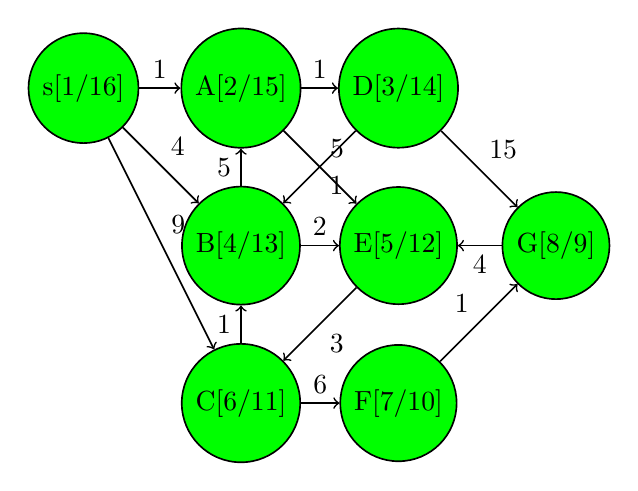
\begin{tikzpicture}[->, semithick,auto, node distance=2cm]


\node[draw, circle, fill=\sfill] (s) at (0,0) {\sdesc};
\node[draw, circle, fill=\Afill] (A) [right of=s] {\Adesc};
\node[draw, circle, fill=\Bfill] (B) [below of=A] {\Bdesc};
\node[draw, circle, fill=\Cfill] (C) [below of=B] {\Cdesc};
\node[draw, circle, fill=\Dfill] (D) [right of=A] {\Ddesc};
\node[draw, circle, fill=\Efill] (E) [below of=D] {\Edesc};
\node[draw, circle, fill=\Ffill] (F) [below of=E] {\Fdesc};
\node[draw, circle, fill=\Gfill] (G) [right of=E] {\Gdesc};

\path 	(s) 	edge node {1} (A)
		edge node {4} (B)
		edge node {9} (C)
	(A) 	edge node {1} (D)
		edge node {5} (E)
	(B) 	edge node {5} (A)
		edge node {2} (E)
	(C) 	edge node {1} (B)
		edge node {6} (F)
	(D) 	edge node {1} (B)
		edge node {15} (G)
	(E) 	edge node {3} (C)
	(F) 	edge node {1} (G)
	(G) 	edge node {4} (E)
	;

\end{tikzpicture}

\\
\gdef\sfill{lightgray}
\gdef\sdesc{s[1/]}
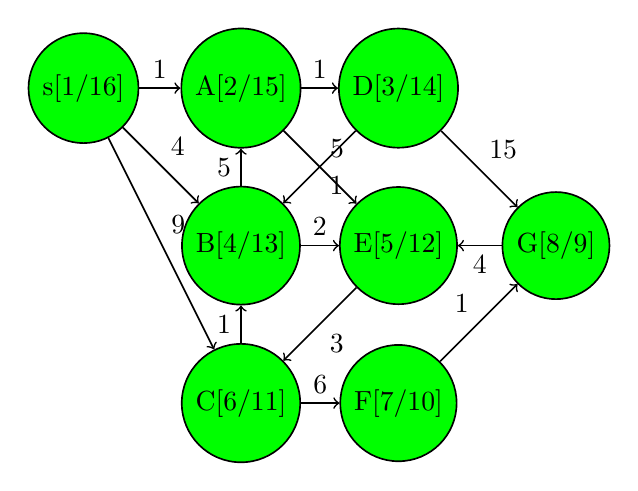
\begin{tikzpicture}[->, semithick,auto, node distance=2cm]


\node[draw, circle, fill=\sfill] (s) at (0,0) {\sdesc};
\node[draw, circle, fill=\Afill] (A) [right of=s] {\Adesc};
\node[draw, circle, fill=\Bfill] (B) [below of=A] {\Bdesc};
\node[draw, circle, fill=\Cfill] (C) [below of=B] {\Cdesc};
\node[draw, circle, fill=\Dfill] (D) [right of=A] {\Ddesc};
\node[draw, circle, fill=\Efill] (E) [below of=D] {\Edesc};
\node[draw, circle, fill=\Ffill] (F) [below of=E] {\Fdesc};
\node[draw, circle, fill=\Gfill] (G) [right of=E] {\Gdesc};

\path 	(s) 	edge node {1} (A)
		edge node {4} (B)
		edge node {9} (C)
	(A) 	edge node {1} (D)
		edge node {5} (E)
	(B) 	edge node {5} (A)
		edge node {2} (E)
	(C) 	edge node {1} (B)
		edge node {6} (F)
	(D) 	edge node {1} (B)
		edge node {15} (G)
	(E) 	edge node {3} (C)
	(F) 	edge node {1} (G)
	(G) 	edge node {4} (E)
	;

\end{tikzpicture}

\\
\gdef\Afill{lightgray}
\gdef\Adesc{A[2/]}
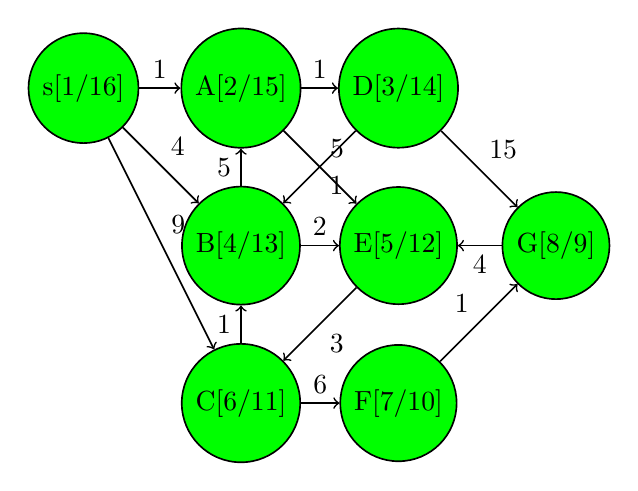
\begin{tikzpicture}[->, semithick,auto, node distance=2cm]


\node[draw, circle, fill=\sfill] (s) at (0,0) {\sdesc};
\node[draw, circle, fill=\Afill] (A) [right of=s] {\Adesc};
\node[draw, circle, fill=\Bfill] (B) [below of=A] {\Bdesc};
\node[draw, circle, fill=\Cfill] (C) [below of=B] {\Cdesc};
\node[draw, circle, fill=\Dfill] (D) [right of=A] {\Ddesc};
\node[draw, circle, fill=\Efill] (E) [below of=D] {\Edesc};
\node[draw, circle, fill=\Ffill] (F) [below of=E] {\Fdesc};
\node[draw, circle, fill=\Gfill] (G) [right of=E] {\Gdesc};

\path 	(s) 	edge node {1} (A)
		edge node {4} (B)
		edge node {9} (C)
	(A) 	edge node {1} (D)
		edge node {5} (E)
	(B) 	edge node {5} (A)
		edge node {2} (E)
	(C) 	edge node {1} (B)
		edge node {6} (F)
	(D) 	edge node {1} (B)
		edge node {15} (G)
	(E) 	edge node {3} (C)
	(F) 	edge node {1} (G)
	(G) 	edge node {4} (E)
	;

\end{tikzpicture}

\\
\gdef\Dfill{lightgray}
\gdef\Ddesc{D[3/]}
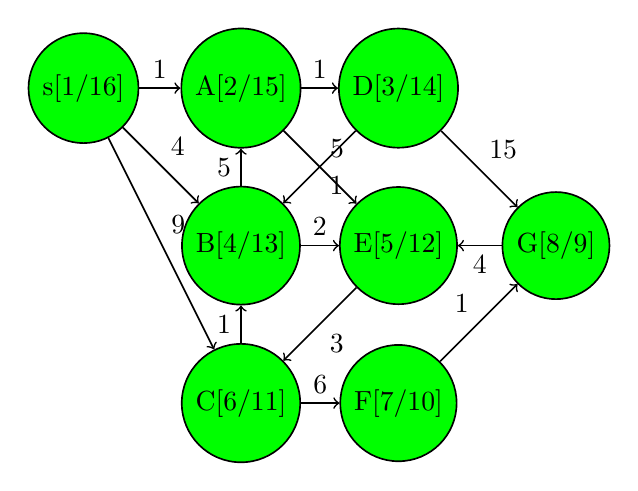
\begin{tikzpicture}[->, semithick,auto, node distance=2cm]


\node[draw, circle, fill=\sfill] (s) at (0,0) {\sdesc};
\node[draw, circle, fill=\Afill] (A) [right of=s] {\Adesc};
\node[draw, circle, fill=\Bfill] (B) [below of=A] {\Bdesc};
\node[draw, circle, fill=\Cfill] (C) [below of=B] {\Cdesc};
\node[draw, circle, fill=\Dfill] (D) [right of=A] {\Ddesc};
\node[draw, circle, fill=\Efill] (E) [below of=D] {\Edesc};
\node[draw, circle, fill=\Ffill] (F) [below of=E] {\Fdesc};
\node[draw, circle, fill=\Gfill] (G) [right of=E] {\Gdesc};

\path 	(s) 	edge node {1} (A)
		edge node {4} (B)
		edge node {9} (C)
	(A) 	edge node {1} (D)
		edge node {5} (E)
	(B) 	edge node {5} (A)
		edge node {2} (E)
	(C) 	edge node {1} (B)
		edge node {6} (F)
	(D) 	edge node {1} (B)
		edge node {15} (G)
	(E) 	edge node {3} (C)
	(F) 	edge node {1} (G)
	(G) 	edge node {4} (E)
	;

\end{tikzpicture}

\\
\gdef\Bfill{lightgray}
\gdef\Bdesc{B[4/]}
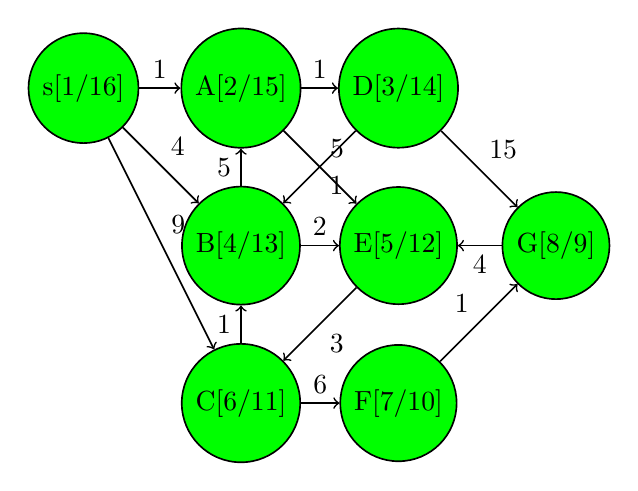
\begin{tikzpicture}[->, semithick,auto, node distance=2cm]


\node[draw, circle, fill=\sfill] (s) at (0,0) {\sdesc};
\node[draw, circle, fill=\Afill] (A) [right of=s] {\Adesc};
\node[draw, circle, fill=\Bfill] (B) [below of=A] {\Bdesc};
\node[draw, circle, fill=\Cfill] (C) [below of=B] {\Cdesc};
\node[draw, circle, fill=\Dfill] (D) [right of=A] {\Ddesc};
\node[draw, circle, fill=\Efill] (E) [below of=D] {\Edesc};
\node[draw, circle, fill=\Ffill] (F) [below of=E] {\Fdesc};
\node[draw, circle, fill=\Gfill] (G) [right of=E] {\Gdesc};

\path 	(s) 	edge node {1} (A)
		edge node {4} (B)
		edge node {9} (C)
	(A) 	edge node {1} (D)
		edge node {5} (E)
	(B) 	edge node {5} (A)
		edge node {2} (E)
	(C) 	edge node {1} (B)
		edge node {6} (F)
	(D) 	edge node {1} (B)
		edge node {15} (G)
	(E) 	edge node {3} (C)
	(F) 	edge node {1} (G)
	(G) 	edge node {4} (E)
	;

\end{tikzpicture}

\\
\gdef\Efill{lightgray}
\gdef\Edesc{E[5/]}
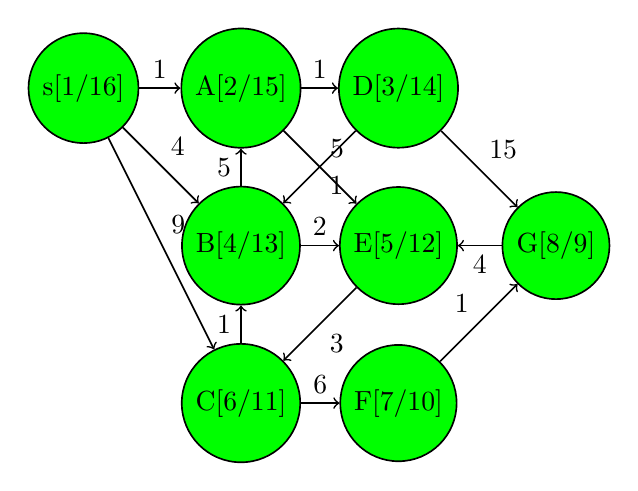
\begin{tikzpicture}[->, semithick,auto, node distance=2cm]


\node[draw, circle, fill=\sfill] (s) at (0,0) {\sdesc};
\node[draw, circle, fill=\Afill] (A) [right of=s] {\Adesc};
\node[draw, circle, fill=\Bfill] (B) [below of=A] {\Bdesc};
\node[draw, circle, fill=\Cfill] (C) [below of=B] {\Cdesc};
\node[draw, circle, fill=\Dfill] (D) [right of=A] {\Ddesc};
\node[draw, circle, fill=\Efill] (E) [below of=D] {\Edesc};
\node[draw, circle, fill=\Ffill] (F) [below of=E] {\Fdesc};
\node[draw, circle, fill=\Gfill] (G) [right of=E] {\Gdesc};

\path 	(s) 	edge node {1} (A)
		edge node {4} (B)
		edge node {9} (C)
	(A) 	edge node {1} (D)
		edge node {5} (E)
	(B) 	edge node {5} (A)
		edge node {2} (E)
	(C) 	edge node {1} (B)
		edge node {6} (F)
	(D) 	edge node {1} (B)
		edge node {15} (G)
	(E) 	edge node {3} (C)
	(F) 	edge node {1} (G)
	(G) 	edge node {4} (E)
	;

\end{tikzpicture}

\\
\gdef\Cfill{lightgray}
\gdef\Cdesc{C[6/]}
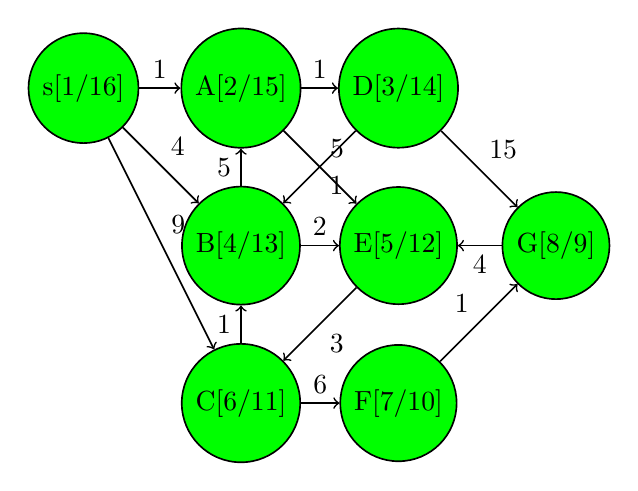
\begin{tikzpicture}[->, semithick,auto, node distance=2cm]


\node[draw, circle, fill=\sfill] (s) at (0,0) {\sdesc};
\node[draw, circle, fill=\Afill] (A) [right of=s] {\Adesc};
\node[draw, circle, fill=\Bfill] (B) [below of=A] {\Bdesc};
\node[draw, circle, fill=\Cfill] (C) [below of=B] {\Cdesc};
\node[draw, circle, fill=\Dfill] (D) [right of=A] {\Ddesc};
\node[draw, circle, fill=\Efill] (E) [below of=D] {\Edesc};
\node[draw, circle, fill=\Ffill] (F) [below of=E] {\Fdesc};
\node[draw, circle, fill=\Gfill] (G) [right of=E] {\Gdesc};

\path 	(s) 	edge node {1} (A)
		edge node {4} (B)
		edge node {9} (C)
	(A) 	edge node {1} (D)
		edge node {5} (E)
	(B) 	edge node {5} (A)
		edge node {2} (E)
	(C) 	edge node {1} (B)
		edge node {6} (F)
	(D) 	edge node {1} (B)
		edge node {15} (G)
	(E) 	edge node {3} (C)
	(F) 	edge node {1} (G)
	(G) 	edge node {4} (E)
	;

\end{tikzpicture}

\\
\gdef\Ffill{lightgray}
\gdef\Fdesc{F[7/]}
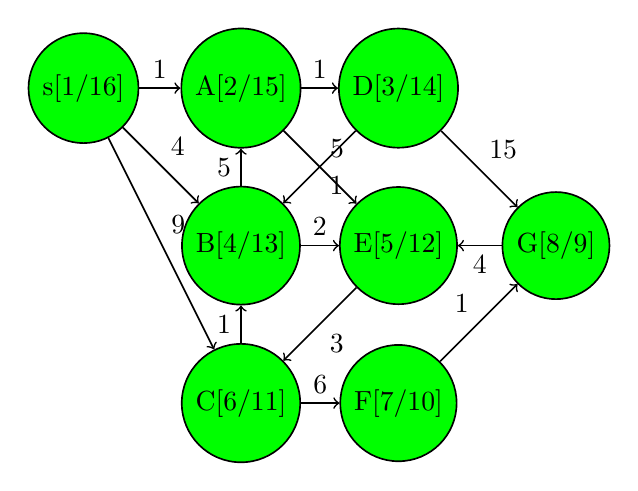
\begin{tikzpicture}[->, semithick,auto, node distance=2cm]


\node[draw, circle, fill=\sfill] (s) at (0,0) {\sdesc};
\node[draw, circle, fill=\Afill] (A) [right of=s] {\Adesc};
\node[draw, circle, fill=\Bfill] (B) [below of=A] {\Bdesc};
\node[draw, circle, fill=\Cfill] (C) [below of=B] {\Cdesc};
\node[draw, circle, fill=\Dfill] (D) [right of=A] {\Ddesc};
\node[draw, circle, fill=\Efill] (E) [below of=D] {\Edesc};
\node[draw, circle, fill=\Ffill] (F) [below of=E] {\Fdesc};
\node[draw, circle, fill=\Gfill] (G) [right of=E] {\Gdesc};

\path 	(s) 	edge node {1} (A)
		edge node {4} (B)
		edge node {9} (C)
	(A) 	edge node {1} (D)
		edge node {5} (E)
	(B) 	edge node {5} (A)
		edge node {2} (E)
	(C) 	edge node {1} (B)
		edge node {6} (F)
	(D) 	edge node {1} (B)
		edge node {15} (G)
	(E) 	edge node {3} (C)
	(F) 	edge node {1} (G)
	(G) 	edge node {4} (E)
	;

\end{tikzpicture}

\\
\gdef\Gfill{lightgray}
\gdef\Gdesc{G[8/]}
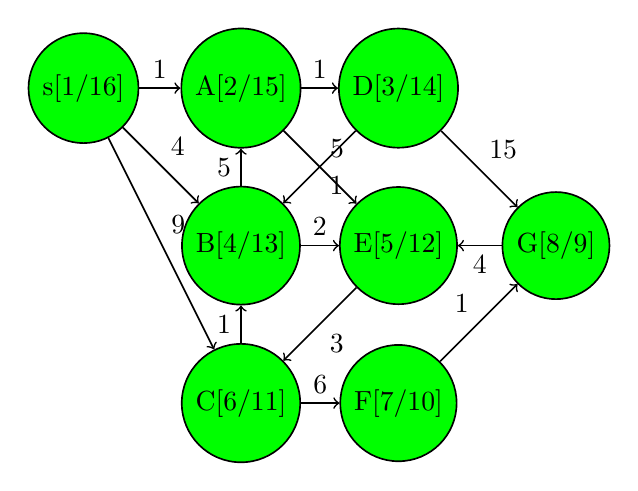
\begin{tikzpicture}[->, semithick,auto, node distance=2cm]


\node[draw, circle, fill=\sfill] (s) at (0,0) {\sdesc};
\node[draw, circle, fill=\Afill] (A) [right of=s] {\Adesc};
\node[draw, circle, fill=\Bfill] (B) [below of=A] {\Bdesc};
\node[draw, circle, fill=\Cfill] (C) [below of=B] {\Cdesc};
\node[draw, circle, fill=\Dfill] (D) [right of=A] {\Ddesc};
\node[draw, circle, fill=\Efill] (E) [below of=D] {\Edesc};
\node[draw, circle, fill=\Ffill] (F) [below of=E] {\Fdesc};
\node[draw, circle, fill=\Gfill] (G) [right of=E] {\Gdesc};

\path 	(s) 	edge node {1} (A)
		edge node {4} (B)
		edge node {9} (C)
	(A) 	edge node {1} (D)
		edge node {5} (E)
	(B) 	edge node {5} (A)
		edge node {2} (E)
	(C) 	edge node {1} (B)
		edge node {6} (F)
	(D) 	edge node {1} (B)
		edge node {15} (G)
	(E) 	edge node {3} (C)
	(F) 	edge node {1} (G)
	(G) 	edge node {4} (E)
	;

\end{tikzpicture}

\\
\gdef\Gfill{green}
\gdef\Gdesc{G[8/9]}
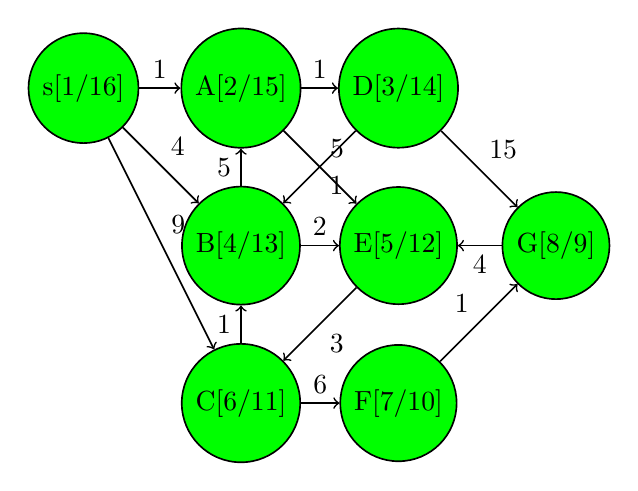
\begin{tikzpicture}[->, semithick,auto, node distance=2cm]


\node[draw, circle, fill=\sfill] (s) at (0,0) {\sdesc};
\node[draw, circle, fill=\Afill] (A) [right of=s] {\Adesc};
\node[draw, circle, fill=\Bfill] (B) [below of=A] {\Bdesc};
\node[draw, circle, fill=\Cfill] (C) [below of=B] {\Cdesc};
\node[draw, circle, fill=\Dfill] (D) [right of=A] {\Ddesc};
\node[draw, circle, fill=\Efill] (E) [below of=D] {\Edesc};
\node[draw, circle, fill=\Ffill] (F) [below of=E] {\Fdesc};
\node[draw, circle, fill=\Gfill] (G) [right of=E] {\Gdesc};

\path 	(s) 	edge node {1} (A)
		edge node {4} (B)
		edge node {9} (C)
	(A) 	edge node {1} (D)
		edge node {5} (E)
	(B) 	edge node {5} (A)
		edge node {2} (E)
	(C) 	edge node {1} (B)
		edge node {6} (F)
	(D) 	edge node {1} (B)
		edge node {15} (G)
	(E) 	edge node {3} (C)
	(F) 	edge node {1} (G)
	(G) 	edge node {4} (E)
	;

\end{tikzpicture}

\\
\gdef\Ffill{green}
\gdef\Fdesc{F[7/10]}
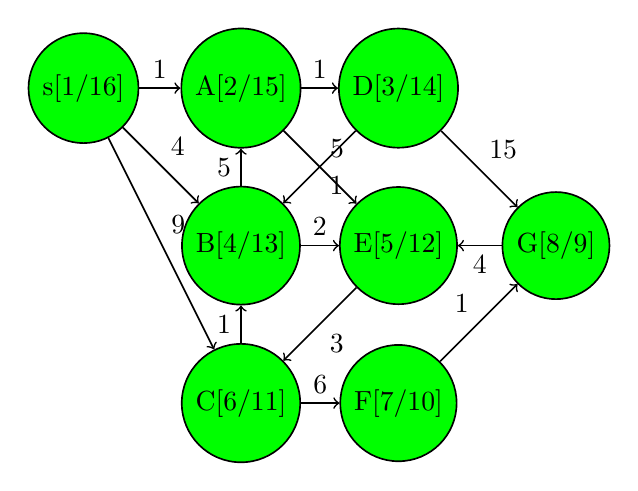
\begin{tikzpicture}[->, semithick,auto, node distance=2cm]


\node[draw, circle, fill=\sfill] (s) at (0,0) {\sdesc};
\node[draw, circle, fill=\Afill] (A) [right of=s] {\Adesc};
\node[draw, circle, fill=\Bfill] (B) [below of=A] {\Bdesc};
\node[draw, circle, fill=\Cfill] (C) [below of=B] {\Cdesc};
\node[draw, circle, fill=\Dfill] (D) [right of=A] {\Ddesc};
\node[draw, circle, fill=\Efill] (E) [below of=D] {\Edesc};
\node[draw, circle, fill=\Ffill] (F) [below of=E] {\Fdesc};
\node[draw, circle, fill=\Gfill] (G) [right of=E] {\Gdesc};

\path 	(s) 	edge node {1} (A)
		edge node {4} (B)
		edge node {9} (C)
	(A) 	edge node {1} (D)
		edge node {5} (E)
	(B) 	edge node {5} (A)
		edge node {2} (E)
	(C) 	edge node {1} (B)
		edge node {6} (F)
	(D) 	edge node {1} (B)
		edge node {15} (G)
	(E) 	edge node {3} (C)
	(F) 	edge node {1} (G)
	(G) 	edge node {4} (E)
	;

\end{tikzpicture}

\\
\gdef\Cfill{green}
\gdef\Cdesc{C[6/11]}
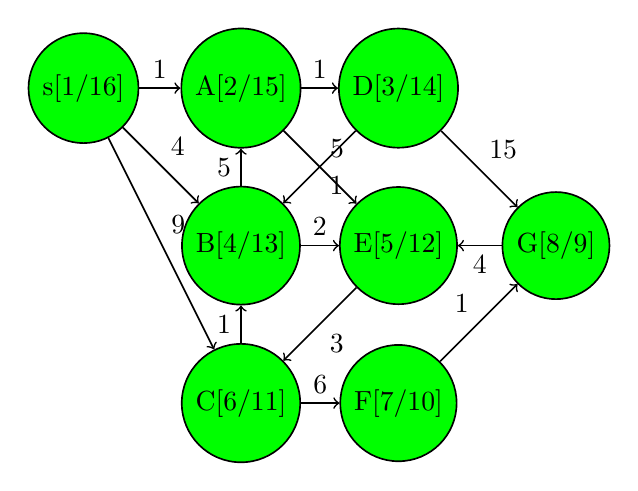
\begin{tikzpicture}[->, semithick,auto, node distance=2cm]


\node[draw, circle, fill=\sfill] (s) at (0,0) {\sdesc};
\node[draw, circle, fill=\Afill] (A) [right of=s] {\Adesc};
\node[draw, circle, fill=\Bfill] (B) [below of=A] {\Bdesc};
\node[draw, circle, fill=\Cfill] (C) [below of=B] {\Cdesc};
\node[draw, circle, fill=\Dfill] (D) [right of=A] {\Ddesc};
\node[draw, circle, fill=\Efill] (E) [below of=D] {\Edesc};
\node[draw, circle, fill=\Ffill] (F) [below of=E] {\Fdesc};
\node[draw, circle, fill=\Gfill] (G) [right of=E] {\Gdesc};

\path 	(s) 	edge node {1} (A)
		edge node {4} (B)
		edge node {9} (C)
	(A) 	edge node {1} (D)
		edge node {5} (E)
	(B) 	edge node {5} (A)
		edge node {2} (E)
	(C) 	edge node {1} (B)
		edge node {6} (F)
	(D) 	edge node {1} (B)
		edge node {15} (G)
	(E) 	edge node {3} (C)
	(F) 	edge node {1} (G)
	(G) 	edge node {4} (E)
	;

\end{tikzpicture}

\\
\gdef\Efill{green}
\gdef\Edesc{E[5/12]}
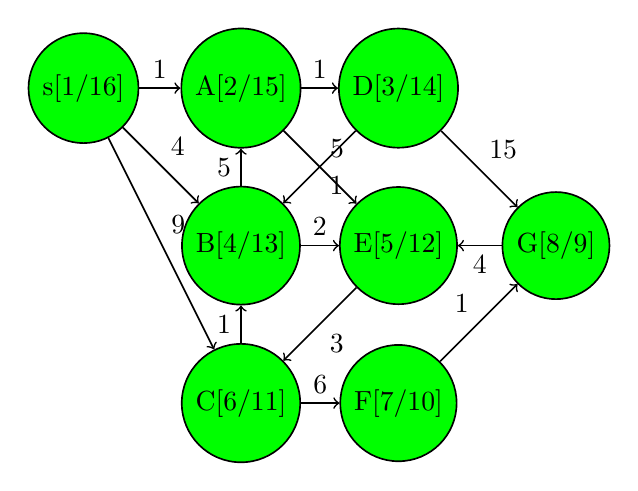
\begin{tikzpicture}[->, semithick,auto, node distance=2cm]


\node[draw, circle, fill=\sfill] (s) at (0,0) {\sdesc};
\node[draw, circle, fill=\Afill] (A) [right of=s] {\Adesc};
\node[draw, circle, fill=\Bfill] (B) [below of=A] {\Bdesc};
\node[draw, circle, fill=\Cfill] (C) [below of=B] {\Cdesc};
\node[draw, circle, fill=\Dfill] (D) [right of=A] {\Ddesc};
\node[draw, circle, fill=\Efill] (E) [below of=D] {\Edesc};
\node[draw, circle, fill=\Ffill] (F) [below of=E] {\Fdesc};
\node[draw, circle, fill=\Gfill] (G) [right of=E] {\Gdesc};

\path 	(s) 	edge node {1} (A)
		edge node {4} (B)
		edge node {9} (C)
	(A) 	edge node {1} (D)
		edge node {5} (E)
	(B) 	edge node {5} (A)
		edge node {2} (E)
	(C) 	edge node {1} (B)
		edge node {6} (F)
	(D) 	edge node {1} (B)
		edge node {15} (G)
	(E) 	edge node {3} (C)
	(F) 	edge node {1} (G)
	(G) 	edge node {4} (E)
	;

\end{tikzpicture}

\\
\gdef\Bfill{green}
\gdef\Bdesc{B[4/13]}
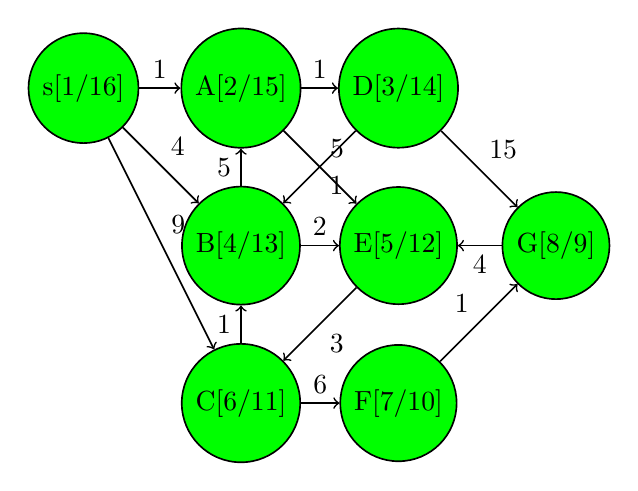
\begin{tikzpicture}[->, semithick,auto, node distance=2cm]


\node[draw, circle, fill=\sfill] (s) at (0,0) {\sdesc};
\node[draw, circle, fill=\Afill] (A) [right of=s] {\Adesc};
\node[draw, circle, fill=\Bfill] (B) [below of=A] {\Bdesc};
\node[draw, circle, fill=\Cfill] (C) [below of=B] {\Cdesc};
\node[draw, circle, fill=\Dfill] (D) [right of=A] {\Ddesc};
\node[draw, circle, fill=\Efill] (E) [below of=D] {\Edesc};
\node[draw, circle, fill=\Ffill] (F) [below of=E] {\Fdesc};
\node[draw, circle, fill=\Gfill] (G) [right of=E] {\Gdesc};

\path 	(s) 	edge node {1} (A)
		edge node {4} (B)
		edge node {9} (C)
	(A) 	edge node {1} (D)
		edge node {5} (E)
	(B) 	edge node {5} (A)
		edge node {2} (E)
	(C) 	edge node {1} (B)
		edge node {6} (F)
	(D) 	edge node {1} (B)
		edge node {15} (G)
	(E) 	edge node {3} (C)
	(F) 	edge node {1} (G)
	(G) 	edge node {4} (E)
	;

\end{tikzpicture}

\\
\gdef\Dfill{green}
\gdef\Ddesc{D[3/14]}
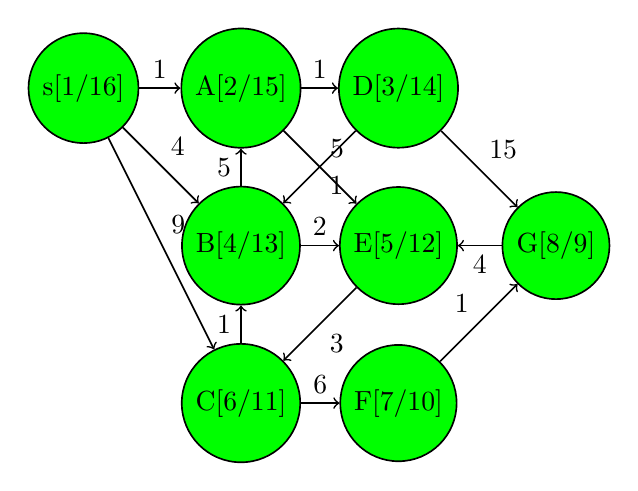
\begin{tikzpicture}[->, semithick,auto, node distance=2cm]


\node[draw, circle, fill=\sfill] (s) at (0,0) {\sdesc};
\node[draw, circle, fill=\Afill] (A) [right of=s] {\Adesc};
\node[draw, circle, fill=\Bfill] (B) [below of=A] {\Bdesc};
\node[draw, circle, fill=\Cfill] (C) [below of=B] {\Cdesc};
\node[draw, circle, fill=\Dfill] (D) [right of=A] {\Ddesc};
\node[draw, circle, fill=\Efill] (E) [below of=D] {\Edesc};
\node[draw, circle, fill=\Ffill] (F) [below of=E] {\Fdesc};
\node[draw, circle, fill=\Gfill] (G) [right of=E] {\Gdesc};

\path 	(s) 	edge node {1} (A)
		edge node {4} (B)
		edge node {9} (C)
	(A) 	edge node {1} (D)
		edge node {5} (E)
	(B) 	edge node {5} (A)
		edge node {2} (E)
	(C) 	edge node {1} (B)
		edge node {6} (F)
	(D) 	edge node {1} (B)
		edge node {15} (G)
	(E) 	edge node {3} (C)
	(F) 	edge node {1} (G)
	(G) 	edge node {4} (E)
	;

\end{tikzpicture}

\\
\gdef\Afill{green}
\gdef\Adesc{A[2/15]}
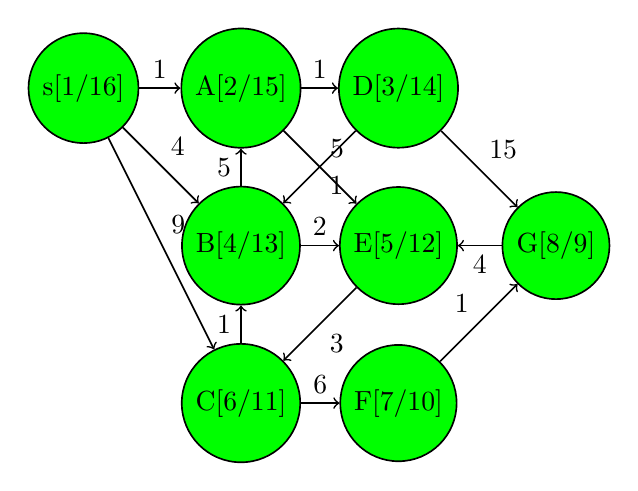
\begin{tikzpicture}[->, semithick,auto, node distance=2cm]


\node[draw, circle, fill=\sfill] (s) at (0,0) {\sdesc};
\node[draw, circle, fill=\Afill] (A) [right of=s] {\Adesc};
\node[draw, circle, fill=\Bfill] (B) [below of=A] {\Bdesc};
\node[draw, circle, fill=\Cfill] (C) [below of=B] {\Cdesc};
\node[draw, circle, fill=\Dfill] (D) [right of=A] {\Ddesc};
\node[draw, circle, fill=\Efill] (E) [below of=D] {\Edesc};
\node[draw, circle, fill=\Ffill] (F) [below of=E] {\Fdesc};
\node[draw, circle, fill=\Gfill] (G) [right of=E] {\Gdesc};

\path 	(s) 	edge node {1} (A)
		edge node {4} (B)
		edge node {9} (C)
	(A) 	edge node {1} (D)
		edge node {5} (E)
	(B) 	edge node {5} (A)
		edge node {2} (E)
	(C) 	edge node {1} (B)
		edge node {6} (F)
	(D) 	edge node {1} (B)
		edge node {15} (G)
	(E) 	edge node {3} (C)
	(F) 	edge node {1} (G)
	(G) 	edge node {4} (E)
	;

\end{tikzpicture}

\\
\gdef\sfill{green}
\gdef\sdesc{s[1/16]}
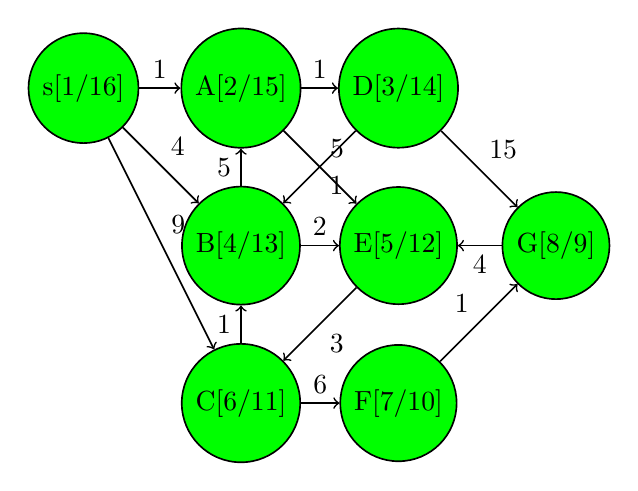
\begin{tikzpicture}[->, semithick,auto, node distance=2cm]


\node[draw, circle, fill=\sfill] (s) at (0,0) {\sdesc};
\node[draw, circle, fill=\Afill] (A) [right of=s] {\Adesc};
\node[draw, circle, fill=\Bfill] (B) [below of=A] {\Bdesc};
\node[draw, circle, fill=\Cfill] (C) [below of=B] {\Cdesc};
\node[draw, circle, fill=\Dfill] (D) [right of=A] {\Ddesc};
\node[draw, circle, fill=\Efill] (E) [below of=D] {\Edesc};
\node[draw, circle, fill=\Ffill] (F) [below of=E] {\Fdesc};
\node[draw, circle, fill=\Gfill] (G) [right of=E] {\Gdesc};

\path 	(s) 	edge node {1} (A)
		edge node {4} (B)
		edge node {9} (C)
	(A) 	edge node {1} (D)
		edge node {5} (E)
	(B) 	edge node {5} (A)
		edge node {2} (E)
	(C) 	edge node {1} (B)
		edge node {6} (F)
	(D) 	edge node {1} (B)
		edge node {15} (G)
	(E) 	edge node {3} (C)
	(F) 	edge node {1} (G)
	(G) 	edge node {4} (E)
	;

\end{tikzpicture}


\end{longtable}
Unser Tiefensuchwald besteht aus genau einem Tiefensuchbaum, der sich wie folgt durch den Graphen windet:\\
$s \to A \to D \to B \to E \to C \to F \to G$\\
Die Rückführung ist genau anders herum.